\documentclass[aspectratio=169,12pt]{beamer}

% ===================================================================
% Package สำหรับภาษาไทย (XeLaTeX)
% ===================================================================
\usepackage{fontspec}
\IfFontExistsTF{TH Sarabun New}{
    \setmainfont{TH Sarabun New}[Scale=1.3]
    \setsansfont{TH Sarabun New}[Scale=1.3]
    \setmonofont{TH Sarabun New}[Scale=1.1]
}{
    \setmainfont{Tahoma}[Scale=1.0]
    \setsansfont{Tahoma}[Scale=1.0]
    \setmonofont{Consolas}[Scale=0.9]
}
\XeTeXlinebreaklocale "th"
\XeTeXlinebreakskip = 0pt plus 1pt minus 1pt

% ===================================================================
% Basic Packages
% ===================================================================
\usepackage{booktabs}
\usepackage{array}
\usepackage{amsmath}
\usepackage{listings}
\usepackage{xcolor}
\usepackage{tikz}
\usepackage{graphicx}
\usetikzlibrary{shapes.geometric, arrows.meta, positioning, fit}

% ===================================================================
% Code Listings Style
% ===================================================================
\lstdefinelanguage{json}{
    basicstyle=\ttfamily\footnotesize,
    stringstyle=\color{red},
    morestring=[b]",
    literate=
     *{:}{{{\color{spumagenta}:}}}{1}
      {,}{{{\color{spumagenta},}}}{1}
      {\{}{{{\color{spumagenta}\{}}}{1}
      {\}}{{{\color{spumagenta}\}}}}{1}
      {[}{{{\color{spumagenta}[}}}{1}
      {]}{{{\color{spumagenta}]}}}{1}
}

\lstdefinelanguage{JavaScript}{
    keywords={const, let, var, if, else, return, function, async, await},
    keywordstyle=\color{spumagenta}\bfseries,
    ndkeywords={Math, JSON, console, log},
    ndkeywordstyle=\color{spudarkpink},
    stringstyle=\color{red},
    commentstyle=\color{gray}\itshape,
    morestring=[b]',
    morestring=[b]",
    morestring=[b]`,
    morecomment=[l]{//}
}

\lstset{
    basicstyle=\ttfamily\footnotesize,
    breaklines=true,
    frame=single,
    framerule=0.5pt,
    rulecolor=\color{spumagenta},
    backgroundcolor=\color{gray!5},
    showstringspaces=false,
    columns=fullflexible,
    keepspaces=true,
    xleftmargin=3pt,
    xrightmargin=3pt,
    aboveskip=8pt,
    belowskip=5pt
}

% ===================================================================
% Theme Configuration
% ===================================================================
\usetheme{Madrid}
\usecolortheme{whale}
\setbeamertemplate{navigation symbols}{}
\setbeamertemplate{footline}[frame number]
\usefonttheme{professionalfonts}

% Colors - SPU Magenta/Pink Theme
\definecolor{spumagenta}{RGB}{198, 0, 126}
\definecolor{spupink}{RGB}{236, 0, 140}
\definecolor{spudarkpink}{RGB}{153, 0, 102}
\definecolor{lightpink}{RGB}{255, 230, 245}
\definecolor{lightgreen}{RGB}{230, 250, 230}
\definecolor{lightyellow}{RGB}{255, 255, 230}
\definecolor{lightblue}{RGB}{230, 245, 255}

\setbeamercolor{title}{fg=white,bg=spumagenta}
\setbeamercolor{frametitle}{fg=white,bg=spumagenta}
\setbeamercolor{structure}{fg=spumagenta}
\setbeamercolor{palette primary}{bg=spumagenta,fg=white}
\setbeamercolor{palette secondary}{bg=spudarkpink,fg=white}
\setbeamercolor{palette tertiary}{bg=spumagenta,fg=white}
\setbeamercolor{palette quaternary}{bg=spudarkpink,fg=white}
\setbeamercolor{block title}{bg=spumagenta,fg=white}
\setbeamercolor{block body}{bg=lightpink}

% ===================================================================
% Title Information
% ===================================================================
\title[Lab 03: LINE Gold Bot]{Lab 03: LINE Gold Price Bot}
\subtitle{Hands-on Workshop}
\author{วิชา n8n Workflow Automation}
\institute{ภาคการศึกษาที่ 2/2568}
\date{}

% ===================================================================
% Document Start
% ===================================================================
\begin{document}

% ===== SLIDE 1: TITLE =====
\begin{frame}
\titlepage
\end{frame}

% ===== SLIDE 2: LAB OVERVIEW =====
\begin{frame}{Lab Overview}

\begin{center}
\colorbox{lightpink}{\textcolor{spumagenta}{\textbf{\Large สร้าง LINE Bot ราคาทอง}}}
\end{center}

\vspace{0.5cm}
\begin{columns}
\column{0.5\textwidth}
\textbf{รายละเอียด:}
\begin{itemize}
    \item เวลา: 3 ชั่วโมง
    \item คะแนน: 100 คะแนน
    \item Tests: 10 ข้อ
\end{itemize}

\column{0.5\textwidth}
\textbf{สิ่งที่ต้องเตรียม:}
\begin{itemize}
    \item LINE Account
    \item Docker Desktop
    \item Terminal/Command Prompt
\end{itemize}
\end{columns}

\end{frame}

% ===== SLIDE 3: GRADING =====
\begin{frame}{เกณฑ์การให้คะแนน}

\begin{table}
\scriptsize
\begin{tabular}{clc}
\toprule
\textbf{Test} & \textbf{ตรวจอะไร} & \textbf{คะแนน} \\
\midrule
1 & มีไฟล์ workflow.json & 10 \\
2 & เป็น valid JSON & 10 \\
3 & มี Webhook Node & 10 \\
4 & Webhook ใช้ POST method & 10 \\
5 & มี HTTP Request Node สำหรับ Gold API & 10 \\
6 & Gold API URL ถูกต้อง & 10 \\
7 & มี Code Node & 10 \\
8 & มี HTTP Request Node สำหรับ LINE Reply & 10 \\
9 & LINE Reply URL ถูกต้อง & 10 \\
10 & มีการจัดรูปแบบข้อความราคาทอง & 10 \\
\midrule
& \textbf{รวม} & \textbf{100} \\
\bottomrule
\end{tabular}
\end{table}

\end{frame}

% ===== SLIDE 4: WORKFLOW OVERVIEW =====
\begin{frame}{Workflow ที่ต้องสร้าง}

\begin{center}
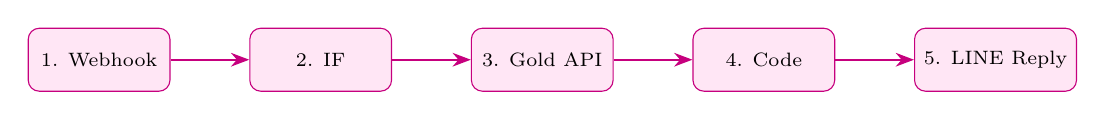
\begin{tikzpicture}[
    node distance=1cm,
    box/.style={rectangle, draw=spumagenta, fill=lightpink, minimum width=1.8cm, minimum height=0.8cm, text centered, rounded corners, font=\scriptsize},
    arrow/.style={->, >=Stealth, thick, spumagenta}
]

\node[box] (webhook) {1. Webhook};
\node[box, right=of webhook] (if) {2. IF};
\node[box, right=of if] (gold) {3. Gold API};
\node[box, right=of gold] (code) {4. Code};
\node[box, right=of code] (line) {5. LINE Reply};

\draw[arrow] (webhook) -- (if);
\draw[arrow] (if) -- (gold);
\draw[arrow] (gold) -- (code);
\draw[arrow] (code) -- (line);

\end{tikzpicture}
\end{center}

\vspace{0.5cm}
\textbf{5 Nodes:}
\begin{enumerate}
    \item \textbf{Webhook} - รับข้อมูลจาก LINE
    \item \textbf{IF} - ตรวจสอบคำสั่ง
    \item \textbf{HTTP Request} - ดึงราคาทอง (GET)
    \item \textbf{Code} - จัดรูปแบบข้อความ
    \item \textbf{HTTP Request} - ส่งข้อความ LINE (POST)
\end{enumerate}

\end{frame}

% ===================================================================
% STEP 1: LINE CHANNEL
% ===================================================================
\section{Step 1: สร้าง LINE Channel}

% ===== SLIDE 5: LINE DEVELOPERS =====
\begin{frame}{Step 1.1: เข้า LINE Developers Console}

\begin{enumerate}
    \item เปิด Browser ไปที่: \texttt{https://developers.line.biz/console/}
    \item คลิก \textbf{Log in with LINE account}
    \item Login ด้วย LINE Account
\end{enumerate}

\vspace{0.5cm}
\begin{center}
\colorbox{lightyellow}{\textcolor{black}{\small ถ้ายังไม่มี Provider ให้สร้างใหม่}}
\end{center}

\end{frame}

% ===== SLIDE 6: CREATE CHANNEL =====
\begin{frame}{Step 1.2: สร้าง Messaging API Channel}

\textbf{ขั้นตอน:}
\begin{enumerate}
    \item เลือก Provider (หรือสร้างใหม่)
    \item คลิก \textbf{Create a new channel}
    \item เลือก \textbf{Messaging API}
    \item กรอกข้อมูล:
    \begin{itemize}
        \item Channel name: \texttt{Gold Price Bot}
        \item Channel description: \texttt{Bot ราคาทอง}
        \item Category: Finance
    \end{itemize}
    \item ติ๊กยอมรับ Terms
    \item คลิก \textbf{Create}
\end{enumerate}

\end{frame}

% ===== SLIDE 7: GET TOKEN =====
\begin{frame}{Step 1.3: Issue Channel Access Token}

\textbf{ขั้นตอน:}
\begin{enumerate}
    \item คลิกที่ Channel ที่สร้าง
    \item ไปที่ \textbf{Messaging API} tab
    \item เลื่อนลงไปที่ \textbf{Channel access token}
    \item คลิก \textbf{Issue}
    \item \textbf{คัดลอก Token เก็บไว้!}
\end{enumerate}

\vspace{0.5cm}
\begin{center}
\colorbox{lightpink}{\textcolor{spumagenta}{\textbf{สำคัญ: เก็บ Token ไว้ใช้ใน n8n}}}
\end{center}

\end{frame}

% ===== SLIDE 8: DISABLE AUTO REPLY =====
\begin{frame}{Step 1.4: ปิด Auto-reply}

\textbf{ขั้นตอน:}
\begin{enumerate}
    \item ในส่วน \textbf{LINE Official Account features}
    \item คลิก \textbf{Edit} ที่ Auto-reply messages
    \item จะเปิดหน้า LINE Official Account Manager
    \item ไปที่ \textbf{ตอบกลับ} > \textbf{การตอบกลับอัตโนมัติ}
    \item \textbf{ปิด} ข้อความตอบกลับอัตโนมัติ
    \item \textbf{ปิด} ข้อความทักทาย
\end{enumerate}

\vspace{0.3cm}
\colorbox{lightyellow}{\textcolor{black}{\small ถ้าไม่ปิด Bot จะตอบซ้ำกับ Auto-reply}}

\end{frame}

% ===================================================================
% STEP 2: NGROK
% ===================================================================
\section{Step 2: ติดตั้ง ngrok}

% ===== SLIDE 9: NGROK SIGNUP =====
\begin{frame}{Step 2.1: สมัคร ngrok}

\textbf{ขั้นตอน:}
\begin{enumerate}
    \item ไปที่ \texttt{https://ngrok.com}
    \item คลิก \textbf{Sign up for free}
    \item สมัครด้วย Email หรือ GitHub/Google
    \item ยืนยัน Email
    \item Login เข้า Dashboard
    \item ไปที่ \textbf{Your Authtoken}
    \item คัดลอก Authtoken
\end{enumerate}

\end{frame}

% ===== SLIDE 10: NGROK INSTALL =====
\begin{frame}[fragile]{Step 2.2: ติดตั้ง ngrok}

\textbf{Windows (Chocolatey):}
\begin{lstlisting}[language=bash]
choco install ngrok
\end{lstlisting}

\textbf{macOS (Homebrew):}
\begin{lstlisting}[language=bash]
brew install ngrok
\end{lstlisting}

\textbf{หรือ Download:}
\begin{itemize}
    \item ดาวน์โหลดจาก \texttt{https://ngrok.com/download}
    \item แตกไฟล์ zip
    \item เพิ่ม path ใน Environment Variables
\end{itemize}

\end{frame}

% ===== SLIDE 11: NGROK CONFIG =====
\begin{frame}[fragile]{Step 2.3: ตั้งค่า ngrok}

\textbf{เพิ่ม Authtoken:}
\begin{lstlisting}[language=bash]
ngrok config add-authtoken YOUR_AUTHTOKEN_HERE
\end{lstlisting}

\vspace{0.5cm}
\textbf{ทดสอบ:}
\begin{lstlisting}[language=bash]
ngrok version
\end{lstlisting}

\vspace{0.3cm}
ถ้าเห็น version number = ติดตั้งสำเร็จ ✅

\end{frame}

% ===================================================================
% STEP 3: RUN N8N + NGROK
% ===================================================================
\section{Step 3: รัน n8n + ngrok}

% ===== SLIDE 12: RUN N8N =====
\begin{frame}[fragile]{Step 3.1: รัน n8n}

\textbf{Terminal 1 - รัน n8n:}
\begin{lstlisting}[language=bash]
docker run -it --rm --name n8n \
  -p 5678:5678 \
  -e N8N_SECURE_COOKIE=false \
  n8nio/n8n
\end{lstlisting}

\vspace{0.5cm}
\textbf{เปิด Browser:}
\begin{lstlisting}
http://localhost:5678
\end{lstlisting}

\end{frame}

% ===== SLIDE 13: RUN NGROK =====
\begin{frame}[fragile]{Step 3.2: รัน ngrok}

\textbf{Terminal 2 - รัน ngrok:}
\begin{lstlisting}[language=bash]
ngrok http 5678
\end{lstlisting}

\vspace{0.5cm}
\textbf{จด URL ที่ได้:}
\begin{lstlisting}
Forwarding  https://abc123.ngrok-free.app -> localhost:5678
\end{lstlisting}

\vspace{0.3cm}
\begin{center}
\colorbox{lightpink}{\textcolor{spumagenta}{\textbf{จด URL นี้ไว้ใช้ตั้งค่า LINE Webhook}}}
\end{center}

\end{frame}

% ===================================================================
% STEP 4: BUILD WORKFLOW
% ===================================================================
\section{Step 4: สร้าง Workflow}

% ===== SLIDE 14: CREATE WORKFLOW =====
\begin{frame}{Step 4.1: สร้าง Workflow ใหม่}

\textbf{ใน n8n:}
\begin{enumerate}
    \item คลิก \textbf{+} หรือ \textbf{Add workflow}
    \item ตั้งชื่อ: \texttt{LINE Gold Price Bot}
\end{enumerate}

\vspace{0.5cm}
\textbf{Nodes ที่ต้องเพิ่ม:}
\begin{enumerate}
    \item Webhook
    \item IF
    \item HTTP Request (Gold API)
    \item Code
    \item HTTP Request (LINE Reply)
\end{enumerate}

\end{frame}

% ===== SLIDE 15: WEBHOOK NODE =====
\begin{frame}[fragile]{Step 4.2: Webhook Node}

\textbf{Settings:}
\begin{itemize}
    \item \textbf{HTTP Method}: POST
    \item \textbf{Path}: \texttt{gold-bot}
\end{itemize}

\vspace{0.5cm}
\textbf{Webhook URL จะเป็น:}
\begin{lstlisting}
https://abc123.ngrok-free.app/webhook/gold-bot
\end{lstlisting}

\vspace{0.3cm}
\colorbox{lightyellow}{\textcolor{black}{\small คลิก "Listen for Test Event" หรือ "Test workflow" ไว้ก่อน}}

\end{frame}

% ===== SLIDE 16: IF NODE =====
\begin{frame}[fragile]{Step 4.3: IF Node (ตรวจสอบคำสั่ง)}

\textbf{ตรวจสอบว่า message มีคำว่า "ราคาทอง" หรือ "gold" หรือ "ทอง"}

\vspace{0.3cm}
\textbf{Conditions (OR):}
\begin{itemize}
    \item \texttt{\{\{ \$json.body.events[0].message.text \}\}} \textbf{contains} \texttt{ราคาทอง}
    \item \texttt{\{\{ \$json.body.events[0].message.text \}\}} \textbf{contains} \texttt{gold}
    \item \texttt{\{\{ \$json.body.events[0].message.text \}\}} \textbf{contains} \texttt{ทอง}
\end{itemize}

\vspace{0.3cm}
\textbf{Combinator}: OR

\end{frame}

% ===== SLIDE 17: GOLD API NODE =====
\begin{frame}[fragile]{Step 4.4: HTTP Request Node (Gold API)}

\textbf{Settings:}
\begin{itemize}
    \item \textbf{Method}: GET
    \item \textbf{URL}: \texttt{https://api.chnwt.dev/thai-gold-api/latest}
\end{itemize}

\vspace{0.5cm}
\textbf{ไม่ต้องตั้งค่าอื่น} - API นี้ไม่ต้อง Authentication

\end{frame}

% ===== SLIDE 18: CODE NODE =====
\begin{frame}[fragile]{Step 4.5: Code Node}

\begin{lstlisting}[language=JavaScript, basicstyle=\ttfamily\scriptsize]
const goldData = $input.first().json;
const webhookData = $('Webhook').first().json;

const lineEvent = webhookData.body.events[0];
const response = goldData.response;

const message = `ราคาทองวันนี้
${response.update_date} ${response.update_time}

ทองคำแท่ง: ขาย ${response.price.gold_bar.sell}
          ซื้อ ${response.price.gold_bar.buy}

ทองรูปพรรณ: ขาย ${response.price.gold.sell}
           ซื้อ ${response.price.gold.buy}`;

return [{
  json: {
    replyToken: lineEvent.replyToken,
    messages: [{ type: "text", text: message }]
  }
}];
\end{lstlisting}

\end{frame}

% ===== SLIDE 19: LINE REPLY NODE =====
\begin{frame}[fragile]{Step 4.6: HTTP Request Node (LINE Reply)}

\textbf{Settings:}
\begin{itemize}
    \item \textbf{Method}: POST
    \item \textbf{URL}: \texttt{https://api.line.me/v2/bot/message/reply}
    \item \textbf{Authentication}: Header Auth
    \item \textbf{Body}: JSON
\end{itemize}

\vspace{0.3cm}
\textbf{Header Auth:}
\begin{itemize}
    \item Name: \texttt{Authorization}
    \item Value: \texttt{Bearer YOUR\_CHANNEL\_ACCESS\_TOKEN}
\end{itemize}

\vspace{0.3cm}
\textbf{Body:} \texttt{\{\{ \$json \}\}}

\end{frame}

% ===== SLIDE 20: CONNECT NODES =====
\begin{frame}{Step 4.7: เชื่อมต่อ Nodes}

\textbf{ลำดับการเชื่อมต่อ:}
\begin{enumerate}
    \item Webhook → IF (main)
    \item IF (true) → HTTP Request (Gold API)
    \item HTTP Request (Gold API) → Code
    \item Code → HTTP Request (LINE Reply)
\end{enumerate}

\vspace{0.5cm}
\begin{center}
\colorbox{lightgreen}{\textcolor{black}{\textbf{บันทึก Workflow!}}}
\end{center}

\end{frame}

% ===================================================================
% STEP 5: CONFIGURE LINE WEBHOOK
% ===================================================================
\section{Step 5: ตั้งค่า LINE Webhook}

% ===== SLIDE 21: SET WEBHOOK URL =====
\begin{frame}[fragile]{Step 5.1: ใส่ Webhook URL ใน LINE}

\textbf{ขั้นตอน:}
\begin{enumerate}
    \item ไปที่ LINE Developers Console
    \item เลือก Channel
    \item ไปที่ \textbf{Messaging API} tab
    \item เลื่อนไปที่ \textbf{Webhook settings}
    \item ใส่ URL:
\end{enumerate}

\begin{lstlisting}
https://YOUR-NGROK-URL.ngrok-free.app/webhook/gold-bot
\end{lstlisting}

\vspace{0.3cm}
\textbf{เปิด} Use webhook = ON

\end{frame}

% ===== SLIDE 22: VERIFY WEBHOOK =====
\begin{frame}{Step 5.2: Verify Webhook}

\textbf{ขั้นตอน:}
\begin{enumerate}
    \item ใน LINE Console คลิก \textbf{Verify}
    \item ถ้าสำเร็จจะเห็น: \textcolor{green}{\textbf{Success}}
\end{enumerate}

\vspace{0.5cm}
\textbf{ถ้า Error:}
\begin{itemize}
    \item ตรวจสอบว่า n8n ทำงานอยู่
    \item ตรวจสอบว่า ngrok ทำงานอยู่
    \item ตรวจสอบ URL ให้ถูกต้อง
    \item ใน n8n ต้องกด Test workflow
\end{itemize}

\end{frame}

% ===================================================================
% STEP 6: TEST
% ===================================================================
\section{Step 6: ทดสอบ}

% ===== SLIDE 23: ADD FRIEND =====
\begin{frame}{Step 6.1: เพิ่ม Bot เป็นเพื่อน}

\textbf{ขั้นตอน:}
\begin{enumerate}
    \item ใน LINE Developers Console
    \item ไปที่ \textbf{Messaging API} tab
    \item สแกน \textbf{QR Code} ด้วย LINE App
    \item เพิ่มเป็นเพื่อน
\end{enumerate}

\end{frame}

% ===== SLIDE 24: SEND MESSAGE =====
\begin{frame}{Step 6.2: ทดสอบส่งข้อความ}

\textbf{ขั้นตอน:}
\begin{enumerate}
    \item เปิด LINE App
    \item เปิดแชทกับ Bot
    \item พิมพ์: \texttt{ราคาทอง}
    \item รอ Bot ตอบกลับ
\end{enumerate}

\vspace{0.5cm}
\textbf{Expected Result:}
\begin{itemize}
    \item Bot ตอบกลับด้วยราคาทองล่าสุด
    \item แสดงราคาทองคำแท่ง + ทองรูปพรรณ
\end{itemize}

\end{frame}

% ===================================================================
% STEP 7: EXPORT & SUBMIT
% ===================================================================
\section{Step 7: Export \& Submit}

% ===== SLIDE 25: EXPORT WORKFLOW =====
\begin{frame}[fragile]{Step 7.1: Export workflow.json}

\textbf{ขั้นตอน:}
\begin{enumerate}
    \item ใน n8n คลิก Menu (⋮) มุมขวาบน
    \item คลิก \textbf{Download}
    \item บันทึกเป็น \texttt{workflow.json}
    \item แทนที่ไฟล์ในโปรเจค
\end{enumerate}

\end{frame}

% ===== SLIDE 26: GIT PUSH =====
\begin{frame}[fragile]{Step 7.2: Push ขึ้น GitHub}

\begin{lstlisting}[language=bash]
# เพิ่มไฟล์
git add workflow.json

# Commit
git commit -m "Add LINE Gold Bot workflow"

# Push
git push origin main
\end{lstlisting}

\vspace{0.5cm}
\begin{center}
\colorbox{lightgreen}{\textcolor{black}{\textbf{รอ Auto-grading ตรวจ!}}}
\end{center}

\end{frame}

% ===== SLIDE 27: CHECKLIST =====
\begin{frame}{Checklist ก่อนส่ง}

\begin{itemize}
    \item[$\square$] สร้าง LINE Channel แล้ว
    \item[$\square$] ได้ Channel Access Token แล้ว
    \item[$\square$] ติดตั้ง ngrok แล้ว
    \item[$\square$] รัน n8n + ngrok ได้
    \item[$\square$] สร้าง Workflow ครบ 5 Nodes
    \item[$\square$] ตั้งค่า Webhook URL ใน LINE แล้ว
    \item[$\square$] ทดสอบส่ง "ราคาทอง" แล้ว Bot ตอบ
    \item[$\square$] Export workflow.json แล้ว
    \item[$\square$] Push ขึ้น GitHub แล้ว
\end{itemize}

\end{frame}

% ===== SLIDE 28: TROUBLESHOOTING =====
\begin{frame}{Troubleshooting}

\textbf{Bot ไม่ตอบกลับ:}
\begin{itemize}
    \item ตรวจสอบว่า ngrok ยังทำงานอยู่
    \item ตรวจสอบ Webhook URL ใน LINE Console
    \item ดู Execution log ใน n8n
\end{itemize}

\vspace{0.3cm}
\textbf{Error 401 Unauthorized:}
\begin{itemize}
    \item ตรวจสอบ Channel Access Token
    \item ตรวจสอบ Header: \texttt{Bearer YOUR\_TOKEN}
\end{itemize}

\vspace{0.3cm}
\textbf{ngrok URL เปลี่ยน:}
\begin{itemize}
    \item อัพเดท Webhook URL ใน LINE Console
    \item Verify อีกครั้ง
\end{itemize}

\end{frame}

% ===== SLIDE 29: Q&A =====
\begin{frame}{Q\&A}

\begin{center}
\Huge{❓}

\vspace{1cm}
\textbf{\Large มีคำถามไหม?}

\vspace{1cm}
\normalsize
ดู README.md สำหรับรายละเอียดเพิ่มเติม

ดู SETUP\_GUIDE.md สำหรับคู่มือตั้งค่า
\end{center}

\end{frame}

% ===== SLIDE 30: GOOD LUCK =====
\begin{frame}

\begin{center}
\Huge{🍀}

\vspace{1cm}
\textbf{\Huge Good Luck!}

\vspace{1cm}
\Large{ขอให้ทำ Lab สำเร็จ!}
\end{center}

\end{frame}

\end{document}
